\documentclass[11pt,a4paper]{article}
\usepackage[T1]{fontenc}
\usepackage{lmodern}
\usepackage[a4paper,margin=23mm,headheight=14pt]{geometry}
\usepackage{amsmath,amssymb,amsthm,mathtools,bm}
\usepackage{booktabs,tabularx,array,microtype,enumitem,xcolor}
\usepackage{tikz}
\usetikzlibrary{arrows.meta,positioning,calc}
\usepackage{fancyhdr,hyperref}
\definecolor{ink}{HTML}{20354D}
\definecolor{blue}{HTML}{245B86}
\definecolor{pale}{HTML}{F0F5F9}
\hypersetup{colorlinks=true,linkcolor=blue,urlcolor=blue,pdfauthor={},pdftitle={Measurement-Free Memory Cost},pdfsubject={An explanatory report},pdfkeywords={}}
\pagestyle{fancy}\fancyhf{}
\fancyhead[L]{\small\color{ink}Measurement-Free Memory Cost}
\fancyhead[R]{\small\color{ink}Explanatory report}
\fancyfoot[C]{\small\thepage}
\renewcommand{\headrulewidth}{0.3pt}
\setlength{\parindent}{0pt}
\setlength{\parskip}{5.5pt plus 1pt}
\setlength{\emergencystretch}{2em}
\setcounter{tocdepth}{1}
\setlist{topsep=3pt,itemsep=2pt,leftmargin=1.5em}
\numberwithin{equation}{section}
\newtheorem{theorem}{Theorem}[section]
\newtheorem{lemma}[theorem]{Lemma}
\theoremstyle{remark}\newtheorem*{remark}{Interpretation}
\newcommand{\id}{\operatorname{id}}
\newcommand{\Tr}{\operatorname{Tr}}
\newcommand{\rank}{\operatorname{rank}}
\newcommand{\supp}{\operatorname{supp}}
\newcommand{\wt}{\operatorname{wt}}
\newcommand{\Span}{\operatorname{span}}
\newcommand{\F}{\mathbb F_2}
\newcommand{\E}{\mathbb E}
\newcommand{\R}{\mathcal R}
\newcommand{\N}{\mathcal N}
\newcommand{\A}{\mathcal A}
\newcommand{\eps}{\epsilon}
\newcommand{\Fe}{F_{\mathrm e}}
\newcommand{\dd}{\delta_{\diamond}}
\newcommand{\Tg}{T/T^{\dagger}}
\newcommand{\xor}{\oplus}
\newcommand{\positive}[1]{\left[#1\right]_+}
\newcommand{\ket}[1]{\lvert#1\rangle}
\newcommand{\bra}[1]{\langle#1\rvert}
\newcommand{\norm}[1]{\left\lVert#1\right\rVert}
\newcommand{\keypoint}[1]{\begin{quote}\color{ink}\textbf{#1}\end{quote}}
\begin{document}
\thispagestyle{empty}
{\color{blue}\large EXPLANATORY REPORT}\par\vspace{8mm}
{\color{ink}\LARGE\bfseries Measurement-Free Memory Cost\par}
\vspace{3mm}
{\large Noisy records, quantum lifetime, and continuing non-Clifford processing\par}
\vspace{6mm}
\textbf{The question.} Suppose every qubit that stores data or a controller record is noisy. Clean replacement states are available, and ideal Clifford operations may be performed between noise rounds. How much additional processing is needed to preserve an unknown quantum state?

With Clifford operations and resets alone, the best possible lifetime grows only logarithmically with physical width. A sufficiently large archive of noisy syndrome records attains this order. At more economical width, preserving high fidelity for long times requires continuing non-Clifford processing. The necessary gate count grows extensively with the logical payload and accumulated noise duration.

\keypoint{Fresh states can remove entropy. They do not, by themselves, supply the coherent processing needed to decide and apply corrections inside this memory.}

The lower bound is complemented by two storage constructions. The first defers nonlinear decoding to the final endpoint and uses exponential noisy width. The second corrects errors during storage, using at most 42 T or T-dagger gates per recovery node. Its width and gate count have an overhead polynomial in the logarithm of the storage and accuracy parameters. The optimum between the lower and upper gate budgets remains open.

Both the converse and the constructions permit ideal global operations between noisy intervals. Storage duration counts noise rounds, separately from elementary gate depth.
\vfill
\begin{tabularx}{\linewidth}{@{}>{\raggedright\arraybackslash\bfseries}p{32mm}X@{}}
Task & Preserve arbitrary unknown quantum information and its reference correlations.\\[3pt]
Resources & Noisy physical width, number of noise rounds, and internal T/T-dagger count.\\[3pt]
Central mechanism & Noise contracts a binary envelope of backward Pauli observables; non-Clifford gates can replenish it only at a bounded rate.\\
\end{tabularx}
\newpage
\tableofcontents
\vspace{4mm}
\textbf{Reading route.} Sections 1--3 define the task and the forgetting mechanism. Sections 4--6 turn that mechanism into a quantitative processing budget. Sections 7--8 explain the two storage constructions. Sections 9--10 compare their resources and state the remaining questions. Section~\ref{sec:guessing} derives an alternative operational premise from a delayed-basis guessing score. The appendix records the finite checks and a compact notation guide.

\textbf{Conventions.} All systems are finite-dimensional. A quantum channel is a completely positive, trace-preserving linear map, abbreviated CPTP. Logarithms written as $\ln$ are natural; $\log_2$ has base two. Probabilities, gate counts, qubit counts, and numbers of rounds are dimensionless. No physical clock time is assigned to a round.

\section{What the memory must preserve}
\subsection{Why a classical record is part of the device}
A classical bit can be copied, compared, and restored by majority voting. An unknown quantum state cannot be copied. Quantum error correction instead extracts a \emph{syndrome}: information about the error that does not reveal the logical amplitudes. A decoder converts that syndrome into a correction.

In an ordinary measured architecture, a protected classical computer may retain syndrome histories and evaluate the correction rule. Here every retained record occupies noisy physical qubits in the memory. Nonlinear processing during storage must be implemented by allowed gates on those registers. Storing the record in the computational basis does not protect it from noise.

The input may be entangled with an external reference, and recovery must retain that entanglement. Preserving a few expectation values or a measured classical description does not solve this task.

\subsection{Width, rounds, and allowed operations}
Let $n$ be the maximum number of physical qubits present during storage, $k\ge1$ the number of logical qubits, and $D\ge0$ the number of noisy rounds. Width includes data, syndrome records, temporary workspace, and controller registers. An inactive slot may be reset before reuse. A preparation device or classical controller that retains information between rounds also belongs to the width.

Each round independently applies the product channel $\N_\gamma^{\otimes n}$, where
\begin{equation}
\N_\gamma(X)=(1-\gamma)X+\gamma\frac I2\Tr X,
\qquad 0<\gamma<1.
\label{eq:noise}
\end{equation}
The argument $X$ in this formula is any single-qubit operator; for a density matrix it has trace one. Set
\begin{equation}
q=1-\gamma,\qquad \kappa=-\ln q>0.
\end{equation}
The parameter $\gamma$ is the probability of \emph{complete depolarization} in this mixture. Equivalently, the Pauli probabilities are $1-3\gamma/4$ for identity and $\gamma/4$ each for $X,Y,Z$. The resulting bit-flip probability for a computational-basis record is $\gamma/2$; it must be distinguished from the depolarization probability.

Between rounds, the fixed circuit may apply arbitrary ideal global Clifford unitaries, replacement resets, and counted T or T-dagger gates. A Clifford unitary maps a Pauli operator to another Pauli under conjugation, up to phase. A T gate is $\operatorname{diag}(1,e^{i\pi/4})$; its inverse is T-dagger. The total number of these internal gates is $m_T$.

A reset on subsystem $A$ is exactly
\begin{equation}
\R_{\tau,A}(X)=\tau_A\otimes\Tr_A X,
\label{eq:reset}
\end{equation}
with the original tensor ordering restored. The replacement state $\tau_A$ is independent of the input and of the retained subsystem. It may be mixed, nonstabilizer, or entangled within $A$. Correlated preparations at different times cannot provide an uncounted memory for the unknown input.

There is no postselection, free external feedback, or data-dependent external schedule. Coherent control is permitted when its registers and gates are counted. Processing between successive noise layers is ideal, so its elementary gate depth does not automatically produce additional noisy rounds.

\subsection{The charged interval and the fidelity criterion}
An arbitrary initial encoder $\mathcal E$ and arbitrary final decoder $\mathcal D$ lie outside the charged storage interval. With storage channel $\Phi_D$, the recovered logical channel is
\begin{equation}
\Lambda=\mathcal D\circ\Phi_D\circ\mathcal E.
\end{equation}
There is no protected quantum bypass between the endpoints. An endpoint may do extensive computation after storage ends; it supplies no protected memory during the preceding rounds.

Let $K=2^k$ and define a normalized maximally entangled state between the logical input and a reference:
\begin{equation}
\ket{\Omega_K}=\frac1{\sqrt K}\sum_{j=1}^K\ket j\ket j.
\end{equation}
The lower bounds assume Bell entanglement fidelity
\begin{equation}
\Fe(\Lambda)=\bra{\Omega_K}(\id\otimes\Lambda)
\bigl(\ket{\Omega_K}\bra{\Omega_K}\bigr)\ket{\Omega_K}
\ge1-\eps.
\label{eq:fidelity}
\end{equation}
This convention uses overlap with the pure target, without taking a square root. The constructions prove the stronger worst-case bound
\begin{equation}
\dd(\Lambda):=\frac12\norm{\Lambda-\id_K}_\diamond\le\eps.
\label{eq:diamond}
\end{equation}
The diamond norm allows an arbitrary reference system: it bounds the trace-norm error of the output even when the input is entangled. Trace distance is half the trace norm, with $\norm X_1=\Tr\sqrt{X^\dagger X}$. Equation~\eqref{eq:diamond} implies \eqref{eq:fidelity}, because a projector onto the target state is a valid measurement effect.

\begin{figure}[ht]
\centering
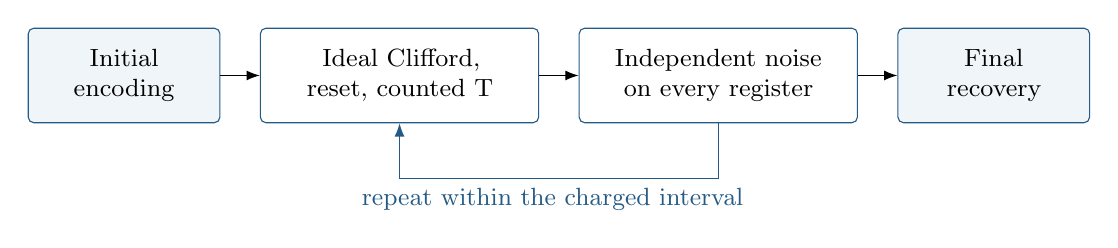
\begin{tikzpicture}[>=Latex,node distance=5mm,
 box/.style={draw=blue,rounded corners=2pt,minimum height=12mm,align=center,font=\small},
 endpoint/.style={box,fill=pale,text width=22mm},
 inner/.style={box,text width=33mm}]
\node[endpoint] (enc) {Initial\\encoding};
\node[inner,right=of enc] (a) {Ideal Clifford,\\reset, counted T};
\node[inner,right=of a] (b) {Independent noise\\on every register};
\node[endpoint,right=of b] (dec) {Final\\recovery};
\draw[->] (enc)--(a);\draw[->] (a)--(b);\draw[->] (b)--(dec);
\draw[->,blue] (b.south) -- ++(0,-7mm) -| node[pos=.26,below,font=\small]{repeat within the charged interval} (a.south);
\end{tikzpicture}
\caption{Every register carrying information between storage rounds is noisy. The repeated interval alternates ideal processing with independent noise on all registers; initial encoding and final recovery lie outside the charged interval.}
\end{figure}

\section{The observable description of memory}
\subsection{Pauli labels are binary vectors}
The single-qubit Pauli matrices $I,X,Y,Z$ form an operator basis. On $n$ qubits, their tensor products form a basis with $4^n$ elements. Ignore global phases and label a Pauli by
\begin{equation}
v=(x,z)\in W_n:=\F^{2n},
\end{equation}
where $(x_j,z_j)$ equals $(0,0),(1,0),(0,1),(1,1)$ for $I,X,Z,Y$, respectively. Adding labels modulo two corresponds to multiplying Paulis up to phase. Their commutation is described by
\begin{equation}
[v,w]=x\cdot z'+z\cdot x'\pmod2,
\qquad w=(x',z').
\end{equation}
A value zero means commuting, and one means anticommuting.

A Clifford acts as an invertible binary linear map preserving this form. It may spread a Pauli over many qubits while retaining a single Pauli label. Backward propagation can therefore bound the number of independent labels through which the input can influence the output.

\subsection{Backward propagation tests input dependence}
For a channel $\Phi$, its adjoint satisfies
\begin{equation}
\Tr[O\Phi(\rho)]=\Tr[\Phi^\dagger(O)\rho].
\end{equation}
Thus $\Phi^\dagger(O)$ identifies which input observables can affect a chosen output measurement. If every output observable pulls back to a scalar multiple of identity, the output is independent of the input. The channel is then a replacement channel $X\mapsto\tau\Tr X$.

The backward calculation propagates all output observables \emph{together}. For an operator $O$, its Pauli support is the set of labels with nonzero coefficients in its Pauli expansion. An envelope $V\le W_n$ is a binary linear subspace containing every support encountered at a cut. Its dimension
\begin{equation}
r=\dim_{\F}V
\end{equation}
counts independent binary labels. It is a proof quantity, not a number of stored logical qubits.

The envelope may contain labels absent from the actual operator supports. A reset can make coefficients vanish and leave a support set that is no longer linear. Enclosing that set in a linear space preserves an upper bound on input dependence without assuming that the surviving support is itself a subspace.

For the full physical output, initialize $V=W_n$, of dimension $2n$. If a particular final decoder is included, a smaller terminal envelope can sometimes be used. We write its dimension as $M\le2n$, and use $M=2n$ unless the decoder gives a proved improvement.

\subsection{How free operations update the envelope}
Clifford conjugation maps $V$ invertibly, preserving its dimension. A reset deletes coordinates of the reset subsystem. Indeed,
\begin{equation}
\R_{\tau,A}^{\dagger}(P_A\otimes P_B)
=\Tr(\tau_A P_A)I_A\otimes P_B.
\label{eq:reset-adjoint}
\end{equation}
Every surviving label is the projection of the original label onto the retained coordinates, even when some scalar coefficients vanish. This projection is linear and cannot increase dimension. An arbitrary joint $\tau_A$, including a magic state, changes the coefficients without adding independent binary labels under the reset.

Complete depolarization on a set $E$ of qubits kills every Pauli with a nonidentity factor on $E$. Let $\pi_E$ retain the two coordinates of the qubits in $E$. The backward envelope becomes
\begin{equation}
V\longmapsto V\cap\ker\pi_E.
\label{eq:intersection}
\end{equation}
An unrecorded Pauli measurement similarly removes anticommuting labels. This extension does not supply an external measurement record or a free adaptive decoder.

\section{Why Clifford processing eventually forgets}
\subsection{Noise as an unobserved random channel}
Equation~\eqref{eq:noise} is a mixture of identity with probability $q$ and complete depolarization with probability $\gamma$. Sampling these choices gives a CPTP circuit whose average is the original noisy channel. The sampled choices are used only in the proof; the memory and decoder receive no corresponding flags.

At one backward noise layer, the set $E$ contains each qubit independently with probability $\gamma$. The expected surviving rank of any fixed $r$-dimensional subspace $V$ obeys
\begin{equation}
\E_E\dim(V\cap\ker\pi_E)\le qr.
\label{eq:contraction}
\end{equation}
Choose a full-row-rank $r\times2n$ binary generator matrix $G$ for $V$, and select $r$ independent columns. Restrict $G$ to the columns belonging to $E$, obtaining $G_E$. Every selected column whose qubit lies in $E$ remains part of an independent subset of $G_E$. If $Z_E$ counts those selected columns, then
\begin{equation}
\rank G_E\ge Z_E,\qquad \E Z_E=\gamma r.
\end{equation}
The two coordinates of a qubit are selected together by the noise, but linearity of expectation does not require their indicators to be independent. Rank--nullity gives
\begin{equation}
\dim(V\cap\ker\pi_E)=r-\rank G_E,
\end{equation}
which proves \eqref{eq:contraction}.

The envelope arriving at a backward noise layer depends only on noise later in forward time. It is therefore independent of the current layer. Conditioning on that envelope lets us iterate the contraction. Clifford operations and resets between layers cannot increase rank.

\subsection{A replacement component gives a reference-stable bound}
For the full storage channel, the terminal envelope has $M=2n$. A smaller decoder-specific $M$ applies to storage followed by that decoder. In this subsection, $\Phi_D$ includes the fixed decoder when that smaller envelope is used; the bound then concerns the decoded storage channel.

With no internal T gates, the final backward rank $r_b$ in sample $b$ satisfies
\begin{equation}
\E_b r_b\le Mq^D.
\end{equation}
Because a positive integer rank is at least one,
\begin{equation}
p:=\Pr(r_b>0)\le\min\{1,Mq^D\}.
\end{equation}
Every branch with $r_b=0$ is exactly a replacement channel. Grouping branches yields
\begin{equation}
\Phi_D=(1-p)\R_{\tau_G}+p\Psi,
\end{equation}
where $\Psi$ is CPTP and $\tau_G$ is the average replacement state on the zero-rank event. Terms of zero weight can simply be omitted.

Fix any input state $\omega_0$ and set $\tau=\Phi_D(\omega_0)$. Then
\begin{equation}
\Phi_D-\R_\tau
=p\bigl(\Psi-\R_{\Psi(\omega_0)}\bigr).
\end{equation}
The diamond distance between any two channels is at most two. Consequently,
\begin{equation}
\boxed{\frac12\norm{\Phi_D-\R_\tau}_\diamond
\le\min\{1,Mq^D\}.}
\label{eq:forget}
\end{equation}
This bound has no reference-dimension prefactor. Arbitrary encoding before storage and decoding afterwards cannot increase diamond distance.

If $M=0$, the decoded channel is already a replacement channel. For $M>0$, a sufficient depth to make the right side at most $\delta\in(0,1)$ is
\begin{equation}
D\ge\frac{\ln(M/\delta)}{\kappa}.
\end{equation}
Taking $M=2n$ gives a lifetime upper bound of order $\gamma^{-1}\ln n$ at weak noise, since $\kappa=\gamma+O(\gamma^2)$ as $\gamma\to0$.

For a recovered logical channel near a replacement, Bell fidelity is at most $4^{-k}+\delta$. A replacement has Bell fidelity exactly $K^{-2}=4^{-k}$, whatever output state it prepares. Hence any fixed fidelity target $F_0>4^{-k}$ is incompatible with arbitrarily long zero-T storage at fixed width.

The Clifford-memory obstruction and the stochastic Pauli approach are established ingredients. The simultaneous-rank argument sharpens the forgetting scale to a single logarithm and makes the reference-stable statement direct. The next sections use the same rank to quantify continuing processing.

\section{High fidelity requires an envelope at every temporal cut}
\subsection{From binary rank to an operator algebra}
For a binary subspace $V$, let
\begin{equation}
\A_V=\Span_{\mathbb C}\{P_v:v\in V\}.
\end{equation}
This is a unital $*$-algebra: products add labels, and adjoints preserve their span. Its complex dimension is $2^r$ because distinct Paulis are linearly independent. Binary dimension $r$ and operator-space dimension $2^r$ must be distinguished.

Suppose a tail channel $\Theta$, including final decoding, has adjoint range inside $\A_V$. Then $\rank_{\mathbb C}\Theta\le2^r$. Composing any CPTP prefix $\Pi$ cannot increase this rank:
\begin{equation}
\rank_{\mathbb C}(\Theta\circ\Pi)\le2^r.
\label{eq:channelrank}
\end{equation}
Here rank refers to the linear map on operators, rather than to an output density matrix or the state representing the channel.

\subsection{The Bell-fidelity bottleneck}
Kraus operators $A_\alpha$ express the action of a channel as a sum of terms $A_\alpha X A_\alpha^\dagger$. For a logical CPTP channel $\Lambda$, the corresponding matrix on the operator space is $\sum_\alpha\overline{A_\alpha}\otimes A_\alpha$, where the bar denotes complex conjugation. Its trace gives
\begin{equation}
\Tr_{\mathrm{sup}}\Lambda
=\sum_\alpha|\Tr A_\alpha|^2
=K^2\Fe(\Lambda).
\end{equation}
Every eigenvalue of a CPTP superoperator has modulus at most one. For example, its powers are trace-norm contractions on Hermitian operators and are uniformly bounded on all operators after decomposing into Hermitian real and imaginary parts. An eigenvalue of modulus greater than one would contradict this boundedness.

The number of nonzero eigenvalues, counted with algebraic multiplicity, is at most the matrix rank, including for a nondiagonalizable channel. Since the superoperator trace is nonnegative,
\begin{equation}
K^2\Fe(\Lambda)
\le\sum_{\lambda\ne0}|\lambda|
\le\rank_{\mathbb C}\Lambda.
\end{equation}
Together with \eqref{eq:channelrank}, this gives the branchwise bound
\begin{equation}
\Fe(\Theta\circ\Pi)\le\min\{1,2^{r-2k}\}.
\label{eq:rankfidelity}
\end{equation}

Now fix any primitive cut, immediately before or after a gate or noise layer. Sample the noise in the future tail and average the earlier noise into the prefix. Independence makes each resulting complete logical map CPTP. Its envelope rank is an integer $r_b$, and its Bell fidelity satisfies \eqref{eq:rankfidelity}.

For every real $r\ge0$,
\begin{equation}
\min\{1,2^{r-2k}\}
\le4^{-k}+(1-4^{-k})\frac r{2k}.
\label{eq:secant}
\end{equation}
On $[0,2k]$, the convex exponential lies below the line connecting its endpoint values. Above $2k$, the line is at least one. Apply this inequality to each branch \emph{before} averaging. Bell fidelity is linear in the channel, so the actual fidelity condition implies
\begin{equation}
R_t:=\E_b r_{b,t}\ge
a:=2k\,\frac{1-\eps-4^{-k}}{1-4^{-k}}>0,
\quad 0\le\eps<1-4^{-k}.
\label{eq:floor}
\end{equation}
The same floor holds at every cut. The expectation $R_t$ need not be an integer, and individual branches may fall below $a$. A large envelope is necessary for fidelity; it is not sufficient to transmit a quantum state.

For one logical qubit, $a=2(1-4\eps/3)$. At $\eps=0.01$, it is approximately $1.9733$. At the replacement-fidelity threshold $\eps=3/4$, the floor vanishes. This example illustrates the floor's fidelity dependence without asserting that any circuit attains it.

\subsection{A complementary test for genuinely quantum information}
The restricted symplectic form on $V$ has even rank $2s$. Its radical consists of labels in $V$ commuting with every label in $V$. If that subspace has dimension $c=r-2s$, a Clifford change of coordinates puts the algebra in the form
\begin{equation}
\A_V\simeq M_{2^s}\otimes\operatorname{Diag}_{2^c}
\otimes I_{2^{n-s-c}}.
\end{equation}
Here $M_d$ denotes all complex $d\times d$ matrices and $\operatorname{Diag}_d$ the diagonal matrices. The first factor can carry a coherent quantum subsystem. The second is classical, and the last carries no observable dependence in this algebra.

This structure has a direct channel interpretation. With symplectic orthogonal complement $V^\perp$, the map
\begin{equation}
\mathcal E_V(X)=\frac1{|V^\perp|}\sum_{w\in V^\perp}P_wXP_w
\end{equation}
is CPTP and retains exactly the Pauli terms labelled by $V$. It is a self-adjoint projection onto $\A_V$. Thus an adjoint-range condition gives $\Theta=\Theta\circ\mathcal E_V$.

After this projection, any joint state with a reference is a mixture of classical sectors, each with at most a $2^s$-dimensional coherent memory factor. A pure state's Schmidt rank is the number of nonzero singular values of its coefficient matrix across the memory--reference split. The projected state has Schmidt number at most $2^s$: it admits a mixture of pure states with Schmidt rank bounded by $2^s$. Local channels cannot increase that number.

Its overlap with $\ket{\Omega_K}$ is therefore at most $\min\{1,2^{s-k}\}$. Indeed, a normalized pure state of Schmidt rank $S$ has a coefficient matrix whose singular values have squared sum one. Their sum is at most $\sqrt S$ by Cauchy--Schwarz, so its squared Bell overlap is at most $S/K$.

In particular, a large commuting algebra has $s=0$ and Bell overlap at most $1/K$. It may retain many classical labels while retaining no entanglement. This complements the stronger scalar floor obtained from total operator rank at small $r$.

\section{The continuing processing lower bound}
\subsection{What one T gate can replenish}
A fixed Pauli-axis rotation $U=e^{i\theta P_w}$ leaves commuting Paulis unchanged. An anticommuting $P_v$ becomes a linear combination with labels $v$ and $v+w$. A safe backward update is
\begin{equation}
V\longmapsto V+\langle w\rangle,\qquad
\dim V'\le\dim V+1.
\end{equation}
A T or T-dagger gate is such a rotation about a single-qubit $Z$ axis, up to global phase. It can add at most one binary generator. A Clifford or reset adds none.

More generally, assign a gate a proved rank-growth charge $b_g$ if its update always satisfies $\dim V'\le\dim V+b_g$. Let $B=\sum_g b_g$. For actual Clifford+T circuits, take $B=m_T$. An arbitrary operation on a specified set of $s_g$ qubits has a safe charge $2s_g$, because the outside labels are unchanged and the inside coordinate space has that dimension. Such a structural charge is not automatically its T count.

\subsection{A logarithmic balance law}
Traverse the circuit backward, starting from rank $M$. Every cut has expected rank $R\ge a$. Noise gives $R'\le qR$. A charged gate gives $R'\le R+b_g$, so
\begin{equation}
\ln R'-\ln R\le\ln(1+b_g/R)\le b_g/a.
\end{equation}
Sum these logarithmic changes over all noise layers and gates. Free operations contribute nonpositive changes. Since the final backward rank is at least $a$,
\begin{equation}
\ln(a/M)\le D\ln q+B/a.
\end{equation}
It follows that
\begin{equation}
\boxed{B\ge a\positive{D\kappa-\ln(M/a)}.}
\label{eq:budget}
\end{equation}
Here $[x]_+=\max\{x,0\}$ and feasibility requires $M\ge a$. Taking $M=2n$ gives the general decoder-independent result.

For T gates individually, their logarithmic increment is at most $\ln(1+1/a)$, giving the refinement
\begin{equation}
m_T\ge
\frac{\positive{D\kappa-\ln(M/a)}}{\ln(1+1/a)}.
\label{eq:integer}
\end{equation}
Round up the right side when using an integer gate count. This refinement and the next section's finite-depth bound may both be imposed.

\subsection{Interpreting the width allowance}
At fixed error bounded away from the replacement threshold, $a=\Theta(k)$. For weak noise, $\kappa\sim\gamma$. Once $D\kappa$ exceeds the width allowance $\ln(2n/a)$ by a fixed factor greater than one, equation~\eqref{eq:budget} requires
\begin{equation}
m_T=\Omega(k\gamma D).
\end{equation}
The bound is extensive in logical payload and accumulated noise duration. The allowance grows as $\ln(n/k)$ for large width-to-payload ratios, but remains nonzero at finite rate when the error tolerance is nonzero. At finite encoding rate $k/n=\Theta(1)$, it corresponds to only $O(1/\gamma)$ rounds at fixed fidelity.

The conclusion does not charge the supply of magic states. Those states are explicitly allowed in replacement resets. It charges internal operations that expand the backward label envelope. Nor does it assert that the lower-bound number of gates is sufficient: an unsuitable code or recovery can fail despite a large gate count.

\section{Finite depth, gate placement, and endpoints}
\subsection{An exact scalar relaxation}
The placement of charged gates gives a sharper finite-depth bound. Number the noise layers in backward order by $j=1,\ldots,D$. Let $b_j$ be the total charge before backward noise layer $j$, and $R_j$ the expected rank just after that layer. With $R_0=M$,
\begin{equation}
R_j\le q(R_{j-1}+b_j),\qquad R_j\ge a.
\end{equation}
Charges after the last backward noise layer remain part of the physical total but cannot relax these earlier constraints.

Introduce a dominating scalar trajectory $x_0=M$, $x_j=q(x_{j-1}+b_j)$. Its feasibility is equivalent to
\begin{equation}
\sum_{i=1}^j q^{j-i+1}b_i\ge a-Mq^j,
\qquad b_i\ge0,\quad j=1,\ldots,D.
\label{eq:scalar}
\end{equation}
Minimizing $\sum_i b_i$ over real injections gives
\begin{align}
\mathcal L(D,M,a,q)
&=\max\left\{0,\max_{1\le h\le D}
\left[\frac aq+(D-h)\frac{(1-q)a}{q}-Mq^{h-1}\right]\right\},
\label{eq:exact}\\
B&\ge\mathcal L(D,M,a,q).
\end{align}
Define $\mathcal L(0,M,a,q)=0$.

The lower certificate follows from a weighted sum of the constraints. Fix an index $h$ and multiply constraint $j$ in \eqref{eq:scalar} by zero for $j<h$, by $(1-q)/q$ for $h\le j<D$, and by $1/q$ for $j=D$. The coefficient on $b_i$ becomes $q^{h-i}$ for $i<h$ and one for $i\ge h$, so it never exceeds one. The right side telescopes to the bracket in \eqref{eq:exact}, certifying that lower bound for every $h$.

A matching feasible scalar trajectory waits until the reserve would fall below $a$, then replenishes only what is needed:
\begin{equation}
b_j=\positive{a/q-x_{j-1}}.
\end{equation}
Write $t_0=\lfloor\ln(M/a)/\kappa\rfloor$. If $D\le t_0$, no injection is necessary in the relaxation. Otherwise the first positive injection is $a/q-Mq^{t_0}$ at layer $t_0+1$, followed by $(1-q)a/q$ per layer. Its total equals the certificate at $h=t_0+1$:
\begin{equation}
\mathcal L=\frac aq-Mq^{t_0}
+(D-t_0-1)\frac{(1-q)a}{q},\qquad D>t_0.
\end{equation}
This also covers equality $Mq^{t_0}=a$: the next layer still needs replenishment.

\keypoint{The scalar optimization is exact for the necessary rank inequalities. It does not construct a physical memory or establish optimal T count.}
Actual ranks are random integers, gate support growth may be smaller than its charge, and a large envelope need not carry quantum information. These additional constraints can only increase the physical optimum.

The physical rank cap $2n$ gives another necessary condition when $D\ge1$:
\begin{equation}
a\le2nq.
\end{equation}
If this fails, the fidelity target is impossible regardless of gate count. In the feasible range $a\le M\le2n$ and $a/q\le2n$, the scalar waiting-and-replenishing trajectory respects the cap. A convenient weaker consequence of \eqref{eq:exact} is
\begin{equation}
B\ge\positive{\frac{(1-q)a}{q}D-(M-a)}.
\end{equation}
At fixed $M,a,q$, the slope of the scalar bound tends to $(1-q)a/q$. This is a statement about the bound; a separate erasure ceiling will prevent indefinite storage at fixed finite width.

\subsection{Every interior interval has its own budget}
Choose two primitive cuts enclosing a contiguous interval $I$. Let $D_I$ count its full noise layers, $B_I$ its internal charge, and $M_I$ a deterministic upper bound on expected decoded-tail envelope rank at its later cut. Boundary gates are assigned according to the cuts so they are counted once. The same global fidelity guarantee supplies the floor $a$ throughout the interval. Its noise is independent of the later suffix, so
\begin{equation}
B_I\ge\mathcal L(D_I,M_I,a,q),\qquad
B_I\ge a\positive{D_I\kappa-\ln(M_I/a)}.
\end{equation}
One can always use $M_I=2n$. Gates in the later suffix can enlarge this envelope beyond the decoder's terminal value $M$, so a smaller terminal reserve cannot automatically be reused inside the interval. Thus gates placed entirely before or after an arbitrarily long interior segment cannot support that segment. The resource requirement concerns timing as well as a total count.

\subsection{Why an arbitrary final decoder changes the reserve}
A decoder with $k$ output qubits need not have terminal support rank $2k$. Define its envelope by taking the binary span of every Pauli label in every pulled-back output Pauli. A single pulled-back observable can have many independent labels.

For example, a decoder measuring three qubits, computing majority, and preparing that output bit obeys
\begin{equation}
\mathcal D^\dagger(Z)
=\tfrac12(Z_1+Z_2+Z_3-Z_1Z_2Z_3).
\end{equation}
Its support spans three independent labels, though it outputs one qubit. The number of output observables is therefore not the dimension of their combined binary support.

For a Clifford decoder followed by discarding unused wires, the $2k$ output generators do pull back to $2k$ independent labels, so $M=2k$ is valid. For arbitrary final decoding, $M=2n$ is the safe choice. Moving nonlinear recovery to the free endpoint is permitted, but its support must be included in that endpoint envelope. Moving it inside the storage interval instead makes its gates part of the charge.

\section{Zero-T storage by retaining a noisy syndrome history}
\subsection{What can be postponed}
Errors in the noise model can also be sampled as independent Pauli labels. In each such history, a stabilizer code occupies a definite syndrome sector. Syndrome extraction can copy that sector label without copying the unknown logical state. If every error increment is correctable and the entire syndrome history can be recovered at the endpoint, physical feedback need not occur during storage.

Branching trees of copies preserve the noisy records until the endpoint, where majority voting and nonlinear decoding are allowed. During storage, the fixed schedule uses only Clifford operations and resets to $\ket0$.

\subsection{A code correcting each noise increment}
Assume $0<\gamma\le1/16$, $k,D\ge1$, and $0<\eps<1$. In this section write the total memory width as $N$ and the data-block width as $n_0$, to distinguish data from archive. Divide the rounds into batches of length at most
\begin{equation}
\tau=\left\lfloor\frac1{16\gamma}\right\rfloor,
\quad J=\left\lceil\frac D\tau\right\rceil,
\quad \Gamma=1-q^\tau\le\frac1{16},
\quad Q=1-\Gamma.
\end{equation}
The final shorter batch has no larger noise. Each data qubit has a nonidentity Pauli increment with probability at most $p_*=3\Gamma/4\le3/64$ per batch.

Stabilizer codes are common $+1$ eigenspaces of independent commuting Pauli generators. With $s$ generators on $n_0$ qubits, the code space has dimension $2^{n_0-s}$ and encodes $k=n_0-s$ qubits. Its distance is the minimum weight of a Pauli that commutes with every generator but acts nontrivially on the encoded state. Weight counts nonidentity tensor factors.

Choose distance at least $2w+1$, with $w=\lfloor n_0/16\rfloor$, so every Pauli of weight at most $w$ is correctable. Set
\begin{align}
R_*&=1-h_2(1/8)-\tfrac18\log_2 3>0,\\
c_\Gamma&=D_{\mathrm{bin}}(1/16\Vert p_*),\\
n_0&=\left\lceil\max\left\{
\frac{k+1}{R_*},\frac{\ln(2J/\eps)}{c_\Gamma}\right\}\right\rceil,
\qquad s=n_0-k.
\label{eq:datawidth}
\end{align}
Here $h_2(u)=-u\log_2u-(1-u)\log_2(1-u)$ and
\begin{equation}
D_{\mathrm{bin}}(u\Vert v)
=u\ln(u/v)+(1-u)\ln[(1-u)/(1-v)]
\end{equation}
is binary relative entropy with natural logarithms. It is positive here because $p_*<1/16$.

A finite counting argument supplies the code. Choose a uniformly random isotropic subspace $S\le\F^{2n_0}$ of dimension $n_0-k$: every pair of its labels commutes. It describes $s$ commuting stabilizers. Symplectic symmetry gives, for any nonzero label $v$,
\begin{equation}
\Pr(v\in S^\perp)
=\frac{2^{n_0+k}-1}{2^{2n_0}-1}
\le\frac43\,2^{k-n_0}.
\end{equation}
The number of Pauli labels of weight at most $2w\le n_0/8$ is at most $2^{n_0(1-R_*)}$. One way to see this is to set $r_*=1/8$ and $y=r_*/[3(1-r_*)]<1$ in the binomial generating function:
\begin{equation}
\sum_{j=0}^{2w}3^j\binom{n_0}j
\le y^{-r_*n_0}(1+3y)^{n_0}
=2^{n_0(1-R_*)}.
\end{equation}
A union bound makes the probability of any nonzero such label in $S^\perp$ at most $(4/3)2^{k-R_*n_0}\le2/3$. A code with the required distance therefore exists.

Let $E_j$ denote the net data Pauli in batch $j$. Its weight has a binomial distribution with parameter at most $p_*$. A Chernoff bound and \eqref{eq:datawidth} give
\begin{equation}
\Pr\{\wt(E_j)>w\}\le e^{-n_0c_\Gamma}\le\frac\eps{2J}.
\end{equation}
Thus all data increments are within the guaranteed correcting radius except with total probability at most $\eps/2$. Code search and final minimum-weight decoding need not be efficient in this existence construction.

\subsection{Extracting records without disturbing the payload}
Let $g_1,\ldots,g_s$ be the stabilizers, and let $\sigma(A)$ record the commutation bits of Pauli $A$ with them. A Clifford encoder $U$ maps input $\ket\psi\ket0^{\otimes s}$ to the code. To obtain $b_{\mathrm{rep}}$ replicas of the current syndrome, decode by $U^\dagger$, copy the $s$ syndrome coordinates by CNOT into fresh zero targets, and reencode by $U$. In every Pauli branch,
\begin{equation}
A\mathcal V\ket\psi\ket0^{\otimes b_{\mathrm{rep}}s}
\longmapsto A\mathcal V\ket\psi\ket{\sigma(A)}^{\otimes b_{\mathrm{rep}}},
\end{equation}
where $\mathcal V$ is the encoding isometry. The formula remains valid with an arbitrary reference attached to $\ket\psi$. The syndrome coordinates are definite computational-basis values conditional on the Pauli history; the logical amplitudes are not copied.

After extraction, records never interact with the data again. They only control CNOTs into fresh record children. Conditional on the data-error history, their dynamics is exactly a classical bit-flip process. Phase flips on disconnected computational-basis records do not affect the recovered bits.

Write $A_j=E_j\cdots E_1$, $\sigma_j=\sigma(A_j)$, and $\sigma_0=0$. At the start of batch $j\ge2$, extract roots encoding $\sigma_{j-1}$. At that same boundary, each old live leaf creates three fresh children and is retired. The children and roots undergo the next batch's noise. There is no archive in batch 1. At the final endpoint, obtain $\sigma_J$ directly from the data. The archive therefore stores precisely the intermediate syndromes $\sigma_1,\ldots,\sigma_{J-1}$.

\subsection{Why noisy trees retain a usable bias}
For each extracted bit, start with $b_{\mathrm{rep}}$ independent replicas. Consider one tree, and let $\eta_h$ be the probability that recursive ternary majority after $h$ further generations misidentifies its \emph{already noisy root}. With $e_*:=\Gamma/2$ and $\eta_0=0$, a child differs from its parent after recursive reconstruction with probability at most $e_*+Q\eta_h$. Three independent children then give
\begin{equation}
\eta_{h+1}\le f_3(e_*+Q\eta_h),\qquad
f_3(u)=3u^2-2u^3.
\end{equation}
If $\eta_h\le1/4$, the argument is at most $(1+\Gamma)/4\le17/64$, and $f_3(17/64)<1/4$. Induction proves $\eta_h\le1/4$ for every age.

The extracted root has already suffered one batch of noise before producing descendants. Including that first noise, the probability of reconstructing the wrong \emph{original extracted bit} is at most
\begin{equation}
e_*+Q/4=\frac12-\frac Q4.
\end{equation}
The distinction matters because the target is the extracted syndrome, before its first noisy batch.

The $b_{\mathrm{rep}}$ replicas use disjoint trees and independent future noise after any slot reuse and reset. Conditional on the data history, their errors are independent. Majority over the replicas has failure probability at most
\begin{equation}
\exp(-b_{\mathrm{rep}}Q^2/8).
\end{equation}
For $J\ge2$, let $H_{\mathrm{arc}}=s(J-1)$ be the number of intermediate syndrome bits to archive. Choose $b_{\mathrm{rep}}$ as the smallest positive odd integer with
\begin{equation}
b_{\mathrm{rep}}\ge\frac8{Q^2}\ln\frac{2H_{\mathrm{arc}}}\eps.
\end{equation}
There are $H_{\mathrm{arc}}$ archived bits, so all records are reconstructed correctly except with probability at most $\eps/2$. For $J=1$, set $b_{\mathrm{rep}}=0$ and omit the archive entirely.

\subsection{Why the history corrects a quantum state}
At the endpoint, reconstruct the intermediate syndromes and form successive differences
\begin{equation}
\widehat\delta_j=\widehat\sigma_j\xor\widehat\sigma_{j-1},
\quad\widehat\sigma_0=0,\quad\widehat\sigma_J=\sigma_J.
\end{equation}
If all archived bits are correct, syndrome linearity makes $\widehat\delta_j=\sigma(E_j)$. Choose a minimum-weight Pauli $C_j$ with that syndrome. On the good data event, $\wt(C_j)\le w$ and $C_j^{-1}E_j$ has zero syndrome and weight at most $2w$, below the code distance. It is consequently a stabilizer up to phase. The product of these representatives cancels the accumulated data error on the logical subspace; Pauli reorderings introduce only global phases.

The final syndrome alone would not identify all correctable increments after many batches. The archive makes their \emph{differences} available, which is why deferred feedback works here.

The joint good event has probability at least $1-\eps$, independent of the logical state. In every good Pauli branch the recovered logical channel is exactly identity. Thus the full recovered channel is
\begin{equation}
\Lambda=(1-\beta)\id+\beta\Lambda_{\mathrm{bad}},
\qquad0\le\beta\le\eps,
\end{equation}
with a CPTP bad-event channel. This proves $\dd(\Lambda)\le\eps$ for arbitrary inputs and references, rather than only for classical codewords.

\subsection{Counting the complete noisy workspace}
Let $L_j$ be the number of live archive leaves after batch $j$. Then
\begin{equation}
L_1=0,\qquad L_j=3L_{j-1}+b_{\mathrm{rep}}s
=\frac{b_{\mathrm{rep}}s}{2}(3^{j-1}-1).
\end{equation}
At a branching boundary, old parents and all fresh targets coexist. Counting only final leaves would miss this overlap. A fixed archive pool of $L_{J-1}+L_J$ slots suffices: reset targets outside the current live set, fan out, then retire the parents. Retired slots remain noisy and can later be reset and reused. The exact total width is
\begin{equation}
N=\begin{cases}
n_0,&J=1,\\
n_0+b_{\mathrm{rep}}s(2\cdot3^{J-2}-1),&J\ge2.
\end{cases}
\end{equation}
All data, roots, leaves, parents, and reuse slots are included. Syndrome extraction and fanout compose to an ideal global Clifford at each batch boundary.

The constants in the coding and tree estimates can be chosen uniformly over $0<\gamma\le1/16$. Since $J\le32\gamma D+1$,
\begin{align}
n_0&=O(k+\ln(J/\eps)),\\
b_{\mathrm{rep}}&=O\!\left(\ln\frac{2J(k+\ln(J/\eps))}\eps\right),\\
N&=O\!\left((k+\ln(J/\eps))
\ln\frac{2J(k+\ln(J/\eps))}\eps\;3^J\right).
\end{align}
For fixed payload and error, $\ln N=O(1+\gamma D)$. Inverting the construction at sufficiently large available width and combining it with \eqref{eq:forget} proves
\begin{equation}
\boxed{D_{\max}(N)=\Theta(\gamma^{-1}\ln N)}
\end{equation}
at fixed $k$ and fixed Bell-fidelity target $4^{-k}<F_0<1$, in the stated weak-noise range. This is sharp lifetime \emph{order}. It does not optimize the width exponent, supply efficient code search, or remove the free final decoder.

\section{Explicit coherent recovery with a charged gate budget}
\subsection{A five-qubit recovery node}
The coherent construction performs nonlinear correction during storage instead of retaining an exponentially growing archive. It uses the five-qubit code with stabilizers
\begin{equation}
g_1=XZZXI,\quad g_2=IXZZX,\quad
g_3=XIXZZ,\quad g_4=ZXIXZ,
\end{equation}
and logical Paulis $\overline X=XXXXX$, $\overline Z=ZZZZZ$. These stabilizers commute and are independent; the two logical Paulis commute with the stabilizers and anticommute with each other.

A Clifford decoder maps the stabilizers to $Z$ on four syndrome wires and the logical pair to $X,Z$ on one remaining wire. Such a map exists by completing them to a symplectic basis. Under a Pauli error $E$, the syndrome wires are $s_1s_2s_3s_4$, where $s_i$ is the commutation bit of $E$ with $g_i$. The logical residual has bits $x(E)=[E,\overline Z]$ and $z(E)=[E,\overline X]$.

The fifteen one-site nonidentity Paulis have distinct nonzero syndromes. Their required logical correction bits are given exactly by the binary polynomials
\begin{align}
f_X(s)&=s_1\xor s_4\xor s_1s_3\xor s_2s_3\xor s_2s_4,\\
f_Z(s)&=s_2\xor s_3\xor s_1s_2\xor s_1s_4\xor s_3s_4.
\label{eq:polynomials}
\end{align}
Products are binary AND and $\xor$ is addition modulo two. Applying $X^{f_X(s)}Z^{f_Z(s)}$ to the decoded logical wire restores every error of weight at most one. The syndrome table in the appendix specifies the finite truth table behind these polynomials.

Each linear term is a Clifford controlled correction. The three quadratic terms of $f_X$ use three Toffoli gates, each applying a NOT when both control qubits are set. Those of $f_Z$ use three controlled-controlled-$Z$ gates. A Hadamard on the target converts between these two three-qubit gates. Their seven-T implementation follows from the integer identity, for bits $u,v,w$,
\begin{align*}
4uvw={}&u+v+w-(u\xor v)-(u\xor w)-(v\xor w)\\
&+(u\xor v\xor w).
\end{align*}
Applying phases $e^{i\pi/4}$ to the four positive parity terms and inverse phases to the three negative terms produces $e^{i\pi uvw}$, precisely a controlled-controlled-$Z$. Each parity can be computed by CNOTs into one of the original wires, phased, and uncomputed before processing the next term. This uses seven T/T-dagger gates and no additional qubit. Thus the recovery has the upper count
\begin{equation}
\boxed{6\times7=42\quad\text{T/T-dagger gates per node}.}
\end{equation}
This is a circuit upper bound, not a minimum. All controls are the original four syndrome wires, and the target is the logical wire. No additional work qubits are required. Reset the syndrome wires after correction; the order of the two conditional logical Paulis changes only a syndrome-dependent phase, irrelevant after those wires are discarded.

For every Pauli error, including uncorrectable ones, this circuit leaves a definite residual logical Pauli. That property is useful for concatenation.

\subsection{Concatenation suppresses the residual error}
Concatenate the code for $L\ge0$ levels. One logical qubit occupies $5^L$ physical qubits. Correct the smallest blocks first, then their parents, up to the root, and reencode using the released and reset syndrome wires. The entire operation uses the original block width. The number of recovery nodes per logical block is
\begin{equation}
1+5+\cdots+5^{L-1}=\frac{5^L-1}{4}.
\end{equation}

Let $p_\ell$ bound the probability of a nonidentity residual at level $\ell$. A parent succeeds whenever at most one of its five children has a residual error. Child error labels depend on disjoint independent physical noise samples, even for entangled logical inputs. A pair union bound gives
\begin{equation}
p_{\ell+1}\le\binom52p_\ell^2=10p_\ell^2,
\qquad
p_L\le\frac{(10p_0)^{2^L}}{10}.
\end{equation}
This deliberately conservative bound does not say that every weight-two error fails.

\subsection{Batching makes the weak-noise dependence explicit}
Assume integers $k,D\ge1$, $0<\eps<1/2$, and $0<\gamma\le1/20$. Choose
\begin{equation}
\tau=\left\lfloor\frac1{20\gamma}\right\rfloor,
\qquad J=\left\lceil\frac D\tau\right\rceil\le40\gamma D+1.
\end{equation}
Perform recovery after every batch, including the last shorter one. A batch of $t\le\tau$ rounds has effective strength $\gamma_t=1-q^t\le t\gamma\le1/20$. Thus $p_0=3\gamma_t/4\le3/80$ and
\begin{equation}
p_L\le\frac1{10}(3/8)^{2^L}.
\end{equation}
Batching gives a cost proportional to $\gamma D+1$ rather than $D$, uniformly at weak noise, because recovery is performed after a batch instead of every arbitrarily short noise step.

For $k$ logical blocks and $J$ recovery batches, the probability of any residual logical error is at most $kJp_L$. Earlier logical Paulis do not change the probability of later, independently sampled errors. The event of no residual error is input-independent and acts as identity on all logical qubits and their reference. As in the archive construction, it gives an identity/bad-event channel mixture and hence $\dd(\Lambda)\le kJp_L$.

\subsection{Finite choices and the achieved resource law}
With these parameters, set
\begin{equation}
A=\max\left\{1,\frac{\ln[kJ/(10\eps)]}{\ln(8/3)}\right\},
\qquad L=\left\lceil\log_2 A\right\rceil.
\end{equation}
Then $kJp_L\le\eps$. The explicit construction satisfies
\begin{equation}
n=k5^L,\qquad
m_T\le42kJ\frac{5^L-1}{4},\qquad
\dd(\Lambda)\le\eps.
\label{eq:explicitupper}
\end{equation}
For $L=0$ the recovery tree is empty and the gate count is zero; the same bound covers this case. Counting the last recovery makes the upper bound conservative and permits a final Clifford decoder.

Let $\alpha=\log_2 5$ and $\ell=1+\ln[k(\gamma D+1)/\eps]$. Since $5^L\le5A^\alpha$,
\begin{equation}
\boxed{n=O(k\ell^\alpha),\qquad
m_T=O\bigl(k(\gamma D+1)\ell^\alpha\bigr).}
\label{eq:upper}
\end{equation}
The constants are uniform over the stated weak-noise range. The achieved bound has a polylogarithmic overhead relative to the extensive lower bound; removing that factor remains open.

For $k=1$, $\gamma=0.01$, $D=1000$, and $\eps=0.01$, the integer prescription gives $n=125$ and $m_T\le260{,}400$. It chooses $\tau=5$, $J=200$, $A\approx7.75$, and $L=3$, with conservative error certificate $20(3/8)^8\approx0.00782$. This example shows the cost of the explicit construction with its loose constants. It gives neither a practical optimum nor an estimate of hardware gate time.

\section{Why more gates still require growing width}
There is a limitation independent of the Clifford restriction. In the identity/depolarization decomposition, one noise layer completely depolarizes all $n$ qubits with probability $\gamma^n$. Once that happens, all correlation with the original unknown input is gone. Input-independent subsequent operations and replacement states cannot restore it.

The probability that this never happens in $D$ independent layers is $(1-\gamma^n)^D$. Every branch containing such a layer is a replacement channel from the logical input and has Bell fidelity $4^{-k}$. Other branches have fidelity at most one. Thus, even with unrestricted internal gates,
\begin{equation}
\boxed{\Fe\le4^{-k}+(1-4^{-k})(1-\gamma^n)^D.}
\label{eq:ceiling}
\end{equation}
For $D\ge1$ and $0<\eps<1-4^{-k}$, put $\eta=\eps/(1-4^{-k})$. High fidelity requires
\begin{equation}
(1-\gamma^n)^D\ge1-\eta.
\end{equation}
Since $1-x\le e^{-x}$, a useful necessary consequence is
\begin{equation}
\gamma^n\le\frac{-\ln(1-\eta)}D,
\quad
n\ge\frac{\ln[D/(-\ln(1-\eta))]}{\ln(1/\gamma)}
\end{equation}
whenever the numerator is positive. For fixed $\gamma$ and small error this is logarithmic width in $D/\eps$. It is an elementary necessary ceiling, not an attainable resource formula.

At any fixed finite width, the right side of \eqref{eq:ceiling} tends to $4^{-k}$ as $D\to\infty$. Consequently, the long-time slope of the processing lower bound must be interpreted along families with adequate growing width, not as a promise of indefinitely reliable storage in one finite device.

\section{What has been established, and what remains open}
The two constructions make different resource choices. The archive retains noisy syndrome history for nonlinear recovery at the endpoint; the coherent construction evaluates corrections during storage. Their guarantees and the necessary resource bounds are compared below.

\begin{table}[ht]
\centering\small
\begin{tabularx}{\linewidth}{@{}>{\raggedright\arraybackslash}p{31mm}>{\raggedright\arraybackslash}X >{\raggedright\arraybackslash}X@{}}
\toprule
Resource choice & Established result & Boundary of the claim\\
\midrule
Clifford and resets only & Sharp lifetime order $\Theta(\gamma^{-1}\ln n)$ at fixed $k,F_0$ & Weak noise; exponential archive width; unrestricted endpoint decoding\\[4pt]
Internal coherent correction & Necessary $\Omega(k\gamma D)$ long-time work; explicit polylogarithmic-overhead upper bound & Optimal T count and width remain open\\[4pt]
Arbitrary internal gates & Full-register depolarization ceiling \eqref{eq:ceiling} & A necessary width condition, not a matching code construction\\
\bottomrule
\end{tabularx}
\caption{The lower bounds, constructions, and ultimate width ceiling answer different parts of the same storage problem.}
\end{table}

The common mechanism is the loss of independent binary directions in the output's dependence on the input. Clifford processing rearranges these directions and resets alter their coefficients, while a T gate can add at most one. High fidelity requires enough directions at every temporal cut, which yields both the total processing budget and its interval version.

The established ingredients include the qualitative memory obstruction, stabilizer and symplectic methods, the algebra and entanglement tools, random-code existence, tree broadcasting, five-qubit coding, concatenation, and exact Toffoli synthesis. The quantitative account developed here lies in the simultaneous envelope contraction, fidelity-dependent and finite-depth budgets, and the fully charged storage constructions. The self-contained derivations are not a claim that every ingredient is new.

Several questions remain. Can coherent coding and decoding remove the power-of-logarithm factor in \eqref{eq:upper}, uniformly as $\gamma\to0$? What is the optimum simultaneous dependence on width, fidelity, payload, and gate placement? Can stronger algebraic information than total envelope rank improve the converse? A lower bound for one particular concatenated decoder would not answer these unrestricted questions.

The present guarantees do not include noisy elementary gates, restricted connectivity, finite processing time, correlated noise, or preparation faults. Both constructions use the stated ideal processing model. A measured protected controller also changes the available resources and requires a separate analysis. These boundaries prevent a direct reinterpretation of $D$ as hardware depth.

\section{A delayed-basis score as an alternative premise}
\label{sec:guessing}
\subsection{The device receives only a quantum challenge}
The same rank ledger can be tested through a classical answer rather than a prescribed Bell-fidelity target. Choose independent uniform strings $X,\Theta\in\{0,1\}^k$ and supply the $k$-qubit state
\[
\ket X_\Theta=\bigotimes_{i=1}^k H^{\Theta_i}\ket{X_i},
\qquad H=\frac1{\sqrt2}\begin{pmatrix}1&1\\1&-1\end{pmatrix}.
\]
Keep $X$ secret and reveal only $\Theta$ after all charged storage. The final decoder may depend arbitrarily on $\Theta$. Let $p=\Pr[\widehat X=X]$ be unconditional \emph{whole-string} success, counting aborts as failures. Write $d=2^k$ and $b_0=1/d$.

The width remains $n$ and the number of independent depolarizing layers remains $D$. Every persistent controller is noisy, counted and processed through the allowed fixed primitives. Counting records does not make arbitrary feedback or data-dependent resets free. Input-independent resets and arbitrary endpoint decoding retain their earlier meaning, without protected side channels or postselection.

Start one common backward envelope at the full physical output \emph{before} basis-dependent readout, with rank $M=2n$. The guessed output length does not reduce this reserve to $2k$.

\subsection{A quantum-plus-classical bottleneck at every cut}
At a cut $t$, average earlier noise into a CPTP prefix $\Pi_t$. An independent future-noise realization $b$ selects a CPTP tail $S_{b,t}$ to the full physical output. The Pauli algebra from Section~4 gives
\[
S_{b,t}=S_{b,t}\mathcal E_V,\qquad
\A_V\simeq M_{2^s}\otimes\operatorname{Diag}_{2^c}\otimes I_G,
\qquad r=2s+c.
\]
The projection $\mathcal E_V$ factors as $J_VF_V$. The CPTP map $F_V$ changes to canonical coordinates, dephases the $c$-bit factor, and discards $G$. The CPTP map $J_V$ reinserts the maximally mixed gauge factor and reverses the coordinates. Thus $F_V\Pi_t$ is a genuine encoder into $s$ quantum qubits and $c$ classical bits. Composing $J_V$ with the tail and final readout reproduces the actual outcome distribution for each basis.

For such an encoder, delayed-basis BB84 guessing obeys
\begin{equation}
p_{b,t}\le\min\{1,\,2^{(s-k)/6},\,2^{s+c-k}\}.
\label{eq:guess-branch}
\end{equation}
The first nontrivial bound permits unlimited classical records. The second uses the finite output dimension: at each fixed basis, $d$ equiprobable output states satisfy $\rho_x\le I$, so their discrimination success is at most $\Tr I/d=2^{s+c-k}$. This count uses the original normalized encoder, before any additional mathematical classical refinement of its states.

The noise flags are proof aids, not information supplied to the device. They select channels independently of the input and basis, so $p=\E_b p_{b,t}$ at every primitive cut. Each branch may be upper-bounded by its optimum decoder without physically revealing a flag.

For $k\ge8$, the two bounds in \eqref{eq:guess-branch} give
\begin{equation}
p_{b,t}\le b_0+(1-b_0)\frac r{2k},\qquad
R_t\ge a_p:=2k\frac{[p-b_0]_+}{1-b_0}.
\label{eq:guess-floor}
\end{equation}
One way to see the first inequality is to maximize the branch bound at fixed $r$. Relaxing $s$ continuously gives $2^{r-k}$ up to $r=5k/6$, then $2^{(r-2k)/7}$ up to $r=2k$, and one thereafter. For $k\ge8$, both convex exponential pieces lie below the chord from $(0,b_0)$ to $(2k,1)$. Averaging that chord proves the floor. For every $k\ge1$, a convenient weaker floor is $k[p-b_0]_+/(1-b_0)$, obtained from the finite-output dimension bound alone. Smaller-block refinements can retain the full concave polygon instead.

\subsection{Processing, timing, and the recovery comparison}
Insert any positive score-derived floor into the earlier balance laws. In particular, \eqref{eq:guess-floor} gives
\begin{equation}
B\ge a_p\positive{D\kappa-\ln(2n/a_p)},\qquad
B\ge\mathcal L(D,2n,a_p,q).
\end{equation}
The individual-T refinement \eqref{eq:integer} also applies. Every contiguous interval has the same global floor, with its own $D_I,B_I$ and entering reserve $M_I\le2n$. Gates outside the interval supply no additional reserve beyond that bound. For $k=12,p=0.4,n=120,\gamma=0.01,D=2000$, the floor is $a_p\simeq9.59648$ and the individual-gate refinement requires at least $171$ internal T/T-dagger gates. This is a necessary condition, not an achievable circuit specification.

The low-score implication should be compared with recovery estimates applied \emph{before} noise averaging. For one complete branch channel, let $F_{\rm rec}$ be its best squared Bell-overlap fidelity, $u$ its average pretty-good guessing success, and $z\ge1/d$ its optimized guessing score. Define
\[
g_d(z)=z^2+\frac{(1-z)^2}{d-1},\qquad
S_\ell=\sum_{j=0}^{\ell}\binom kj.
\]
Established discrimination and recovery estimates give
\begin{align}
g_d(z)&\le u,\qquad F_{\rm rec}\ge z/d,\notag\\
u&\le\frac{1+F_{\rm pg}}2,\qquad
u\le S_\ell F_{\rm pg}+2^{-\ell-1}\mathbf1_{\ell<k},
\quad 0\le\ell\le k,
\label{eq:guess-recovery}
\end{align}
where $F_{\rm pg}\le F_{\rm rec}$ is the squared fidelity of pretty-good recovery. For example, at $z=1/2$ the choice $\ell=2$ already gives a positive recovery-fidelity lower bound of order $k^{-2}$. Each branch also has $F_{\rm rec}\le\min\{1,2^{r-2k}\}$. Combining these inequalities branchwise and then averaging reproduces \eqref{eq:guess-floor} for every $k\ge9$. Thus the direct factorization gives a short operational corollary; low-score applicability alone establishes no additional large-block processing law.

At chance $p=b_0$, discarding the challenge and guessing needs zero gates. Full-register replacement gives $p\le b_0+(1-b_0)(1-\gamma^n)^D$, regardless of gates. The score does not verify noise, controller or side-channel premises. It can witness processing to retain classical as well as quantum information. A remote-preparation wrapper needs its own model- and resource-preserving reduction.

\clearpage
\appendix
\section{Finite identities, verification, and notation}
\subsection{The five-qubit correction truth table}
The following table uses syndrome order $s_1s_2s_3s_4$ and the logical representatives specified in Section 8. $X_j,Y_j,Z_j$ act on physical qubit $j$. The two right columns are the values of \eqref{eq:polynomials}. Listing all sixteen correctable cases fixes the correction rule without a free classical lookup during storage.

\begin{center}
\begin{tabular}{@{}cccc@{}}
\toprule
Syndrome & Error & $f_X$ & $f_Z$\\
\midrule
0000 & $I$ & 0 & 0\\
1000 & $X_2$ & 1 & 0\\
0100 & $Z_5$ & 0 & 1\\
1100 & $X_3$ & 1 & 0\\
0010 & $Z_3$ & 0 & 1\\
1010 & $Z_1$ & 0 & 1\\
0110 & $X_4$ & 1 & 0\\
1110 & $Y_3$ & 1 & 1\\
0001 & $X_1$ & 1 & 0\\
1001 & $Z_4$ & 0 & 1\\
0101 & $Z_2$ & 0 & 1\\
1101 & $Y_2$ & 1 & 1\\
0011 & $X_5$ & 1 & 0\\
1011 & $Y_1$ & 1 & 1\\
0111 & $Y_5$ & 1 & 1\\
1111 & $Y_4$ & 1 & 1\\
\bottomrule
\end{tabular}
\end{center}

\subsection{What finite checks establish}
Deterministic finite calculations check the identities most exposed to sign, support, and scheduling mistakes. They enumerate all 67 binary Pauli subspace algebras on two qubits, test channel-rank and support-growth identities, and compare 1,944 exact-rational scalar optimization certificates. Separate checks cover 4,096 three-increment correctable Pauli histories, 12,315 small-tree noise patterns, first-root noise, and simultaneous parent/child workspace allocation.

The five-qubit calculation evaluates every one of the $4^5=1024$ Pauli errors, checks the correction polynomials, and finds the numbers of errors leaving a nonidentity logical residual at physical weights zero through five:
\begin{equation}
[0,\ 0,\ 90,\ 210,\ 270,\ 198].
\end{equation}
In particular, all weight-zero and weight-one errors are corrected. Integer batching and concatenation parameters are checked in 240 finite cases.

These checks support the finite algebra and circuits. They do not prove an asymptotic statement by extrapolation. General forgetting follows from the envelope induction; the processing converse follows from channel-rank and scalar inequalities; arbitrary-depth archives and concatenation follow from their conditioning and induction arguments. No finite test establishes optimality of 42 gates, an optimal hardware threshold, or attainment of the scalar relaxation by a memory circuit.

\subsection{Boundary cases}
If $D=0$, an identity memory on $k$ qubits suffices. If $\gamma=0$, it suffices for any finite duration; the positive-noise batching formulas need not be used. If $k=0$, the task is vacuous. The constructions state nonzero error tolerance: exact zero error is not asserted under nonzero depolarization. The archive case $J=1$ uses no archived record, and the concatenated construction $L=0$ uses no recovery node.

\subsection{Notation guide}
\begin{tabularx}{\linewidth}{@{}p{25mm}X@{}}
\toprule
Symbol & Meaning\\
\midrule
$n$ & Total noisy width; called $N$ in the archive construction.\\
$k$, $K=2^k$ & Logical qubit count and logical Hilbert-space dimension.\\
$D$, $\gamma$ & Number of full noise layers and complete-depolarization strength.\\
$q$, $\kappa$ & $1-\gamma$ and $-\ln q$.\\
$m_T$ & Number of internal physical T and T-dagger gates.\\
$V$, $r$ & Binary Pauli envelope and its binary dimension.\\
$\A_V$ & Complex Pauli algebra, of dimension $2^r$.\\
$M$ & Terminal envelope dimension, at most $2n$.\\
$M_I$ & Upper bound on expected decoded-tail envelope rank at an interval's later cut.\\
$R_t$, $a$, $a_p$ & Expected envelope rank and its fidelity- or guessing-score-derived floor.\\
$B$, $b_{\mathrm{rep}}$ & Total structural rank-growth charge and number of archive root replicas, respectively.\\
$\tau$, $J$ & Batch length and number of batches; constants differ between the two constructions.\\
$n_0$, $s$ & Archive data-block width and number of its stabilizer generators.\\
$H_{\mathrm{arc}}$ & Number $s(J-1)$ of intermediate syndrome bits to archive.\\
$L$ & Concatenation level of the five-qubit code.\\
\bottomrule
\end{tabularx}
\end{document}

